%%%%%%%%%%%%%%%%%%%%%%%%%%%%%%%%%%%%%%%%%%%%%%%%%%%%%%%%%%%%%%%%%%%%%%%%%%%%%%%%%%%%%
%																					%
%	TRABAJO: Paper Mejoras en el procesador de Redes de Petri						%
%																					%
%		Titulo: 	Soft Core parametrizable con procesamiento de Redes de Petri	%
%																					%
%		Autores:	Julian Nonino													%
%					Carlos Renzo Pisetta											%
%					Orlando Micolini												%
%																					%
%	Seccion: CRECIMIENTO DEL IP CORE												%	
%	Archivo: crecimiento_ip_core.tex												%
%																					%
%%%%%%%%%%%%%%%%%%%%%%%%%%%%%%%%%%%%%%%%%%%%%%%%%%%%%%%%%%%%%%%%%%%%%%%%%%%%%%%%%%%%%

\section{Crecimiento del IP Core}
		Una vez visto el correcto funcionamiento del IP Core, se evalu� el crecimiento del procesador 
		en funci�n de los par�metros que posee. Para esto se generaron procesadores de 8x8, 16x16, 
		32x32,4 8x48 y 64x64 con capacidad de 7 bits por plaza y elementos temporales de 48 bits
		 y se graficaron los valores que se pueden observar en la Figura \ref{fig:resultados09}.
		\begin{figure}[h]
			\centering
			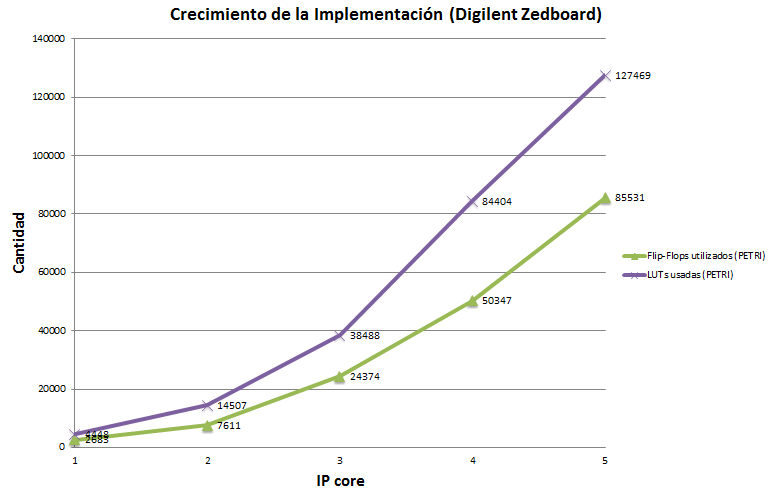
\includegraphics[width=3in]{resultados09}
			\caption{Diferentes implementaciones del procesador de Redes de Petri}
			\label{fig:resultados09}
		\end{figure}
	
		Es posible ver que el crecimiento del IP Core no es algo para despreciar, puesto que 
		se incrementa r�pidamente a medida que aumentamos el tama�o de elementos soportados.
		Se observa tambi�n que si bien la pendiente aumenta, �stos incrementos son cada vez menores,
		tendiendo a linealizar para los IP Cores m�s grandes.
		
		Tambien podemos observar los elementos disponibles que tenemos en una determinada FPGA, para este
		caso una Spartan6 de Xilinx. Vemos que desarrollar una implementacion de 32x32 es inalcansable, en este
		caso es necesario pasar a una con mas recursos. 
